\documentclass[a4paper,12pt]{report}
\addtolength{\oddsidemargin}{-1.cm}
\addtolength{\textwidth}{2cm}
\addtolength{\topmargin}{-2cm}
\addtolength{\textheight}{3.5cm}
\newcommand{\HRule}{\rule{\linewidth}{0.5mm}}
\setcounter{secnumdepth}{5}
\setcounter{tocdepth}{3}
\makeindex

\usepackage{longtable}
\usepackage{graphicx}
\usepackage{makeidx}
\usepackage{hyperref}
\usepackage{verbatim}
\usepackage{placeins}

\hypersetup{
    colorlinks=true,
    linkcolor=blue,
    filecolor=magenta,      
    urlcolor=cyan,
}


% define the title
\author{Ambitious Design}
\title{ Software Requirements Specifications and Technology Neutral Process Design}
\begin{document}
\setlength{\parskip}{6pt}

% generates the title
\begin{titlepage}

\begin{center}
% Upper part of the page           
\textsc{\LARGE Willburg Outdoor PTY(ltd.)}\\[1.5cm]
\textsc{\Large Smart Image Identifier }\\[1.0cm]
\textsc{\Large Version 1.0 }\\[0.5cm]
% Title
\HRule \\[0.4cm]
{ \huge \bfseries  Application Requirements Specifications and Design}\\[0.4cm]
\HRule \\[0.4cm]
% Author and supervisor
\begin{minipage}{0.4\textwidth}
\begin{flushleft} \large
\emph{Author:}\\
Stephen {Swanepoel}
\end{flushleft}
\end{minipage}
\begin{minipage}{0.4\textwidth}
\begin{flushright} \large
\emph{} \\
u11032091
\end{flushright}
\end{minipage}
\begin{minipage}{0.4\textwidth}
\begin{flushleft} \large
Dian {Veldsman}
\end{flushleft}
\end{minipage}
\begin{minipage}{0.4\textwidth}
\begin{flushright} \large
\emph{} \\
u12081095
\end{flushright}
\end{minipage}
\end{minipage}


{\large \today}
\end{center}
\end{titlepage}
\footnotesize
\normalsize

\renewcommand{\thesection}{\arabic{section}}
\newpage

\section {Background}
\\Willburg Outdoor is company that is passionate about South Africa. With this passion comes the need to protect its farmers and it animals from those who intend to harm them. The client intends to use the system to assist in fighting the following problems: animal poaching and farm attacks. 
Willburg provides its' clients with a camera system which is interfaced with a dashboard as well as a mobile application. The cameras snap pictures when movement is detected and sends them to the Willburg server. The images are then pushed to the respective users. Willburg intend on providing its' users with real-time push notifications when a human has been detected in an image captured by a camera on their property. Smart Image Identifier will play an influential role in the prevention of both farm attacks as well as poaching.

\subsection {Smart Image Identification System}
The Smart Image Identifier will consist of 3 modules:
	\begin {itemize}
		\item Manipulating.  
		\item Identification.
		\item Sorting.
	\end {itemize}

The above mentioned module will consist of the following:
	\subsubsection {Manipulating}
		This module consists of:
			\begin {itemize}
				\item Processing an image inorder to prepare it for human identification.
			\end {itemize}

	\subsubsection {Identification}
		This module consists of:
			\begin {itemize}
				\item Identifiying the presence of humans within the image.
			\end {itemize}

	\subsubsection {Sorting}
		This module consists of:
			\begin {itemize}
				\item Sorting of images into baskets and groupings.
			\end {itemize}


\section {Vision and Objectives}
	\subsection {Vision}
	 The client for this project, Willburg Outdoor PTY(ltd.), has called for the design of an application that will assess an image and identify any human(s) present in the image. If a human has been identified by the system, a response will be sent to the Willburg server afterwhich a notification is pushed through to the user. The main idea behind the project is to be able to alert users of Willburg's software that a human has been identified and action can be taken if there is an intruder on the premesis.

	\subsection {Objectives}
	Objectives of the Smart Image Identifier are:
	\begin {itemize}
		\item Identify the presence of a human in the image.
		\item Assesses, store and sort images into a database based on their content.
	\end {itemize}


\section {Process Image}
The ImageProcessing module provides the functionality of manipulating and processing an image inorder for the system to better detect  humans by providing it with multiple tests which it is required to pass.
	\FloatBarrier
	\subsection {Scope}
		The scope of the ImageProcessing module include:
			\begin {itemize}
				\item Submit image to be processed.
				\item Process image.
			\end {itemize}

	\FloatBarrier
	\subsection {Domain Model}
		The image processor uses an image inorder to create an instance of the processed image.
		\begin{figure}[htb]
			\centering
			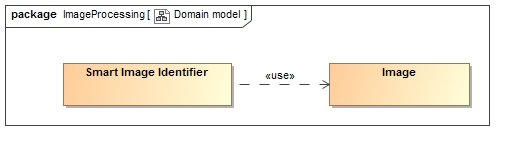
\includegraphics [scale=0.5]{../Diagrams/ProcessImage_Domain_model.jpg}
			\caption{Domain model for the Process Image model}
		\end{figure}	

		\FloatBarrier
		\subsubsection {Service contract}
			\begin{figure}[htb]
				\centering
				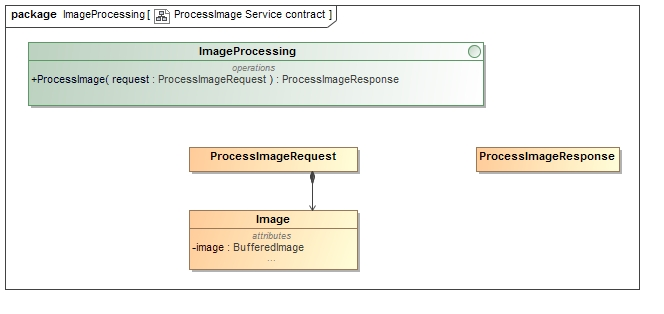
\includegraphics [scale=0.5]{../Diagrams/ProcessImage_Service_contract.jpg}
				\caption{ImageProcessing service contract}
			\end{figure}	
			To process an image the following must hold:
			\begin {itemize}
				\item The dimensions of the image should be large enough to process, at least 600x600.
			\end {itemize}

			If an error occurs during reading the image an IOException is thrown. In addition, the service will be refused if the request does not comply to the data structure specification.
		
		\FloatBarrier
		\paragraph {Functional requirements}

		\FloatBarrier
		\paragraph {processDesign}
		An image is first processed into a buffered image. The buffered image's data is then stored within a Mat object which is then used to manipulate the pixels found in the image. Manipulations include: scaling to a size which is ideal for processing, greyscaling and equalization inorder to better improve the detection of a person. The processed image is then sent as request to identify the presence of a human.
		\begin{figure}[htb]
			\centering
			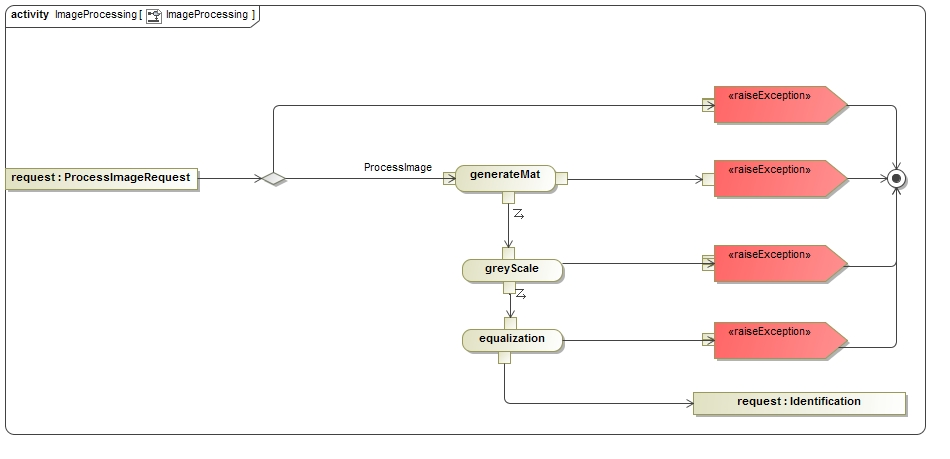
\includegraphics [scale=0.5]{../Diagrams/ImageProcessing.jpg}
			\caption{Process image process design}
		\end{figure}	

\FloatBarrier	
\section {Identification}
The Identification module provides the functionality of identification of humans with OpenCV

	\FloatBarrier	
	\subsection {Scope}
	The scope of the Identification module include:
		\begin {itemize}
			\item Submitting a processed image to perform the identification.
			\item Identify the presence of humans.
		\end {itemize}

	\FloatBarrier	
	\subsection {Domain Model}
		The processed image is sent to the identification module where the OpenCV's built in algorithm is used (HOG - Histogram of Oriented Gradients) and set to the default "people detector".
		\begin{figure}[htb]
			\centering
			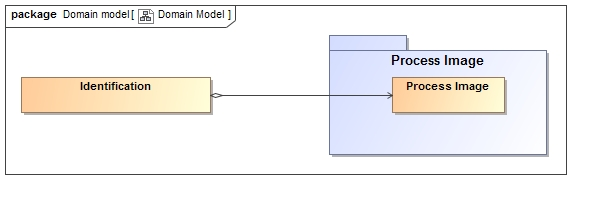
\includegraphics [scale=0.5]{../Diagrams/Identification_Domain_Model.jpg}
			\caption{Identification Domain model}
		\end{figure}	

		\FloatBarrier	
		\subsubsection {Service contract}
			\begin{figure}[htb]
				\centering
				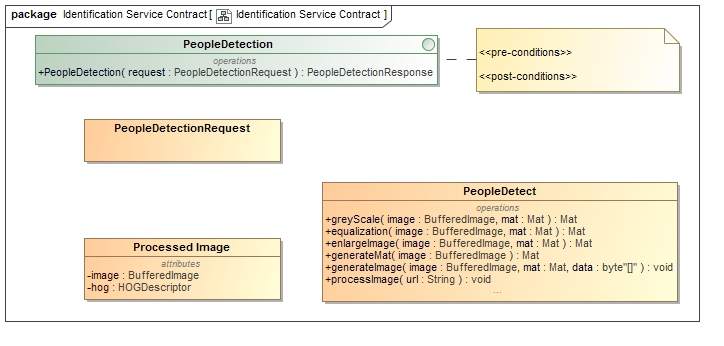
\includegraphics [scale=0.5]{../Diagrams/Identification_Service_Contract.jpg}
				\caption{Identification process design}
			\end{figure}	

			\FloatBarrier				
			\paragraph {Functional requirements}
			
			\FloatBarrier	
			\paragraph {processDesign}
				\begin{figure}[htb]
					\centering
					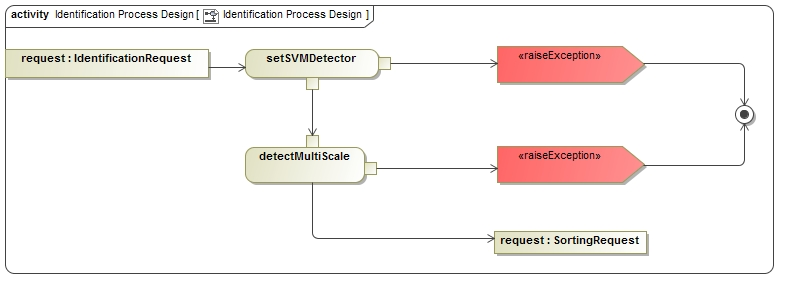
\includegraphics [scale=0.5]{../Diagrams/Identification_Process_Design.jpg}
					\caption{Identification process design}
				\end{figure}	

\section {ImageSorting}
		\FloatBarrier	
		\subsection {Scope}
		The scope of the ImageSorting module include:
			\begin {itemize}
				\item Submit image to be processed.
				\item Process image.
			\end {itemize}
	
	\FloatBarrier		
	\subsection {Domain Model}
		\FloatBarrier	
		\subsubsection {Service contract}		
		\begin{figure}[htb]
			\centering
			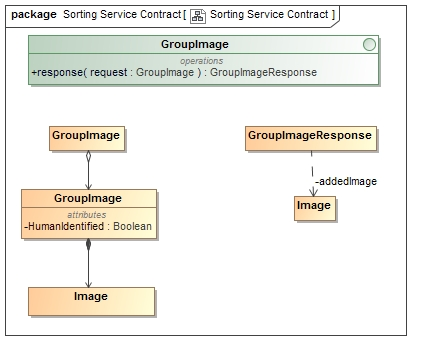
\includegraphics [scale=0.5]{../Diagrams/Sorting_Service_Contract.jpg}
			\caption{Identification process design}
		\end{figure}
		
			\FloatBarrier	
			\paragraph {Functional requirements}

			\FloatBarrier	
			\paragraph {processDesign}
			\begin{figure}[htb]
				\centering
				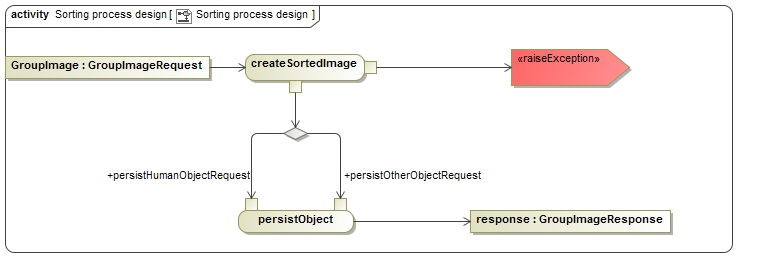
\includegraphics [scale=0.5]{../Diagrams/Sorting_process_design.jpg}
				\caption{Identification process design}
			\end{figure}	



\end{document}
